
\documentclass[8pt]{article}
\usepackage[a4paper,margin=0.5in]{geometry}
\usepackage[utf8]{inputenc}
\usepackage{authblk}
\usepackage{multicol}
\usepackage{ragged2e}
\usepackage{babel}
\usepackage{graphicx}
\usepackage[inline]{enumitem}
\DeclareUnicodeCharacter{00AB}{\guillemotleft}
\usepackage{float}
\usepackage{xcolor}
\usepackage{amsmath}
\usepackage{amsfonts}
\usepackage{caption}
\usepackage{subcaption}
\usepackage[colorlinks=true,linkcolor=blue,urlcolor=blue,citecolor=blue]{hyperref}

\setcounter{secnumdepth}{4}

\title{
\raggedright
Structural bioinformatics \\
\textbf{SAINT: self-attention augmented inception-insideinception network improves protein secondary structure
prediction}}
\author{
    \raggedright
    Mostofa Rafid Uddin\textsuperscript{1,2,†},
    Sazan Mahbub\textsuperscript{1,†},
    M. Saifur Rahman\textsuperscript{1},
    Md Shamsuzzoha Bayzid\textsuperscript{1,*}\\
    \vspace{0.5cm}
    \textsuperscript{1}Department of Computer Science and Engineering, Bangladesh University of Engineering and Technology, Dhaka 1205, Bangladesh and
    \textsuperscript{2}Department of Computer Science and Engineering, East West University, Dhaka 1212, Bangladesh\\
    \vspace{0.3cm}
    *To whom correspondence should be addressed.\\
    Associate Editor: Arne Elofsson\\
    \vspace{0.3cm}
    \textsuperscript{†}The authors wish it to be known that, in their opinion, the first two authors should be regarded as Joint First Authors.\\
    Associate Editor: Arne Elofsson\\
    Received on December 7, 2019; revised on May 10, 2020; editorial decision on May 12, 2020; accepted on May 16, 2020\\
}
\date{}
\usepackage[style=authoryear]{natbib}


\bibliographystyle{plainnat}
\begin{document}

\maketitle
\renewenvironment{abstract}%
{\noindent\textbf{\abstractname}\hspace{1em}}%
{\par}
\begin{abstract}
\newline
\textbf{Motivation: }: Protein structures provide basic insight into how they can interact with other proteins, their functions and biological roles in an organism. Experimental methods (e.g. X-ray crystallography and nuclear magnetic resonance spectroscopy) for predicting the secondary structure (SS) of proteins are very expensive and time consuming. Therefore, developing efficient computational approaches for predicting the SS of protein is of utmost importance. Advances in developing
highly accurate SS prediction methods have mostly been focused on 3-class (Q3) structure prediction. However, 8-class
(Q8) resolution of SS contains more useful information and is much more challenging than the Q3 prediction.\\
\textbf{Results: } We present SAINT, a highly accurate method for Q8 structure prediction, which incorporates self-attention mechanism (a concept from natural language processing) with the Deep Inception-Inside-Inception network in order to effectively capture both the short- and long-range interactions among the amino acid residues. SAINT offers a more interpretable framework than the typical black-box deep neural network methods. Through an extensive evaluation study, we report the performance of SAINT in comparison with the existing best methods on a collection of benchmark datasets, namely, TEST2016, TEST2018, CASP12 and CASP13. Our results suggest that self-attention
mechanism improves the prediction accuracy and outperforms the existing best alternate methods. SAINT is the first of its kind and offers the best known Q8 accuracy. Thus, we believe SAINT represents a major step toward the
accurate and reliable prediction of SSs of proteins.\\

\textbf{Availability and implementation: }SAINT is freely available as an open-source project at https://github.com/
SAINTProtein/SAINT.

\textbf{Contact: }shams.bayzid@gmail.com
\end{abstract}
\rule{\linewidth}{3pt}
\begin{multicols}{2}
\section{Introduction}

Proteins are bio-molecules made of long chains of amino acid residues
connected by peptide bonds. The functions of proteins are usually
determined by their tertiary structure and for determining the tertiary
structure and related properties, the secondary structure (SS) information is crucial. Protein structure can be experimentally determined by
X-ray crystallography and multi-dimensional magnetic resonance in
laboratory, but these methods are very costly and time consuming
and are yet to be consistent with the proliferation of protein sequence
data \citet{jiang2017protein} . Thus, the proteins with known primary
sequence continue to outnumber the proteins with experimentally
determined SSs. The structural properties of a protein depend on its
primary sequence (\citet{anfinsen1973principles}; \citet{baker2001protein}; \citet{bradley2005toward}; \citet{dill2008protein}, yet it remains as a difficult task to accurately determine the secondary and tertiary structures of proteins.
Hence, the problem of predicting the structures of a protein — given
its primary sequence — is crucially important and remains as one of
the greatest challenges in computational biology.
SS — a conformation of the local structure of the polypeptide
backbone — prediction dates back to the work of Pauling and
Corey in 1951 \citet{pauling1951structure} The SSs of proteins are



\section{Approach}
\subsection{Feature representation}

SAINT takes a protein sequence feature vector  $ X = (x_1, x_2, x_3, \dots , x_N)$ as input, where $x_i$ is the vector corresponding to
the $i$th residue, and it returns the protein structure label sequence
vector $Y =  (y_1, y_2, y_3, \dots , y_N) $ as output, where $y_i$ is the structure
label (one of the eight possible states) of the $i$th residue. Similar to
SPOT-1D-base and MUFOLD-SS, our base model contains 57 features from PSSM profiles, HHM profiles and physicochemical properties. To generate PSSM, PSI-BLAST \citet{altschul1997gapped} was run
against Uniref90 database \citet{uniprot2007universal} with inclusion threshold 0.001 and three iterations. The HHM profiles were
generated using HHblits \citet{remmert2012hhblits} using default
parameters against uniprot20\_2013\_03 sequence database. HHblits
also generates seven transition probabilities and three local alignment diversity values, which we used as features as well. Seven physicochemical properties of each amino acid [e.g. steric parameters
(graph-shape index), polarizability, normalized van der Waals volume, hydrophobicity, isoelectric point, helix probability and sheet
probability] were obtained from \citet{meiler2001generation} . So, in our base
model, the dimension of $x_i$ is 57 as this is the concatenation of
$ x_b b m_i \in  \mathbb{R}^{d_{bbm}} (d_{bbm} = 30) $ and $ x_{pss} m_i \in  \mathbb{R}^{d_{pssm}} (d_{pssm} = 20) $ and  $ x_{physica} l_i \in  \mathbb{R}^{d_{physical}} (d_{physical} = 7) $ Additional features were generated
by windowing the predicted contact information as was done in
SPOT-1D. The contact maps were generated using SPOT-Contact
\citet{hanson2018accurate} and were used as our features by varying window lengths (the number of preceding or succeeding residues whose
pairwise contact information were extracted for a target residue).
Our ensemble model constitutes of four different models, that we
trained with varying input features: one without the contact maps
(base model) and three with different window lengths (10, 20 and
50) of the contact-map-based features. The features were normalized to ensure 0 mean and SD of 1 in the training data, similar to
SPOT-1D.

\subsection{Architecture of SAINT}

The architecture of SAINT can be split into three separate discussions:

\begin{enumerate*}[label=(\roman*)]
\item { the architecture of our proposed self-attention module,}
\item { the architecture of the existing inception module and the proposed
attention-augmented inception module and finally}
\item { the overall
pipeline of SAINT.}
\end{enumerate*}


\subsubsection{Self-attention module}
Attention mechanism implies paying attention to specific parts of input data or features while generating output sequence (\cite{bahdanau2014neural};\cite{vaswani2017attention}). It calculates a probability distribution over the elements in the input sequence and then takes the
weighted sum of those elements based on this probability distribution while generating outputs. \\

In self-attention mechanism (\cite{cheng2016long}; \cite{parikh2016decomposable}; \cite{vaswani2017attention}), each vector in the input sequence is
transformed into three vectors- \textit{query, key} and \textit{value}, by three different functions. Each of the output vectors is a weighted sum of the
\textit{value} vectors, where the weights are calculated based on the compatibility of the \textit{query} vectors with the key vectors by a special function, called compatibility function (discussed later in this section).
The self-attention module, we designed and augmented with the
Deep3I network (\cite{fang2018mufold}) is inspired from the selfattention module proposed by \cite{vaswani2017attention} and is depicted
in Figure \ref{fig:picture1}. Our self-attention module takes two inputs:

\begin{enumerate*}[label=(\roman*)]
\item {  the features from the previous inception module or layer, $ x \in  \mathbb{R}^{d_{protein} * d_{feature}} $
and}
\item { position identifiers, $ pos_i d \in \mathbb{R}^{d}_{
protein} $, where $d_{protein}$ is the
length of the protein sequence and $d_{feature}$ is the length of the feature
vector}
\end{enumerate*}
\paragraph{Positional Encoding Sub-module}


 The objective of positional encodings is to inject some information about the relative or
absolute positions of the residues in a protein sequence. The
Positional Encoding PosEnc$_p$ for a position $_p$ can be defined as follows \cite{vaswani2017attention}

\begin{equation}
PosEnc_{p,2i} = \sin(p/1000^{2i/d_{feature}})
\end{equation}
\begin{equation}
PosEnc_{p,2i+1}  = \cos(p/1000^{2i/d_{feature}})
\end{equation}
where $i$ is the dimension. We used such function as it may allow the
model to easily learn to attend by relative positions since for any
fixed offset $k$, PosEnc$_{p+k}$ can be represented as a linear function of
PosEnc$_p$ \cite{vaswani2017attention}. For every position $p$, PosEnc$_p$ has
the dimension $d_{protein} x d_{feature}$. The output of positional encoding is
added with the inputs $x$, resulting in new representations $b$ [see Equation
\eqref{eq:example})], which contain not only the information extracted by
the former layers or modules, but also the information about individual positions
\begin{equation}
b_{pos} = x_{pos} + PosEnc_{pos}
\label{eq:example}
\end{equation}

\paragraph{Scaled dot-product attention sub-module}
The input features in this sub-module, $b \in \mathbb{R}^{d_{protein} * d_{feature}} $  are first transformed into
three feature spaces Q, K and V, representing query, key and value,
respectively, in order to compute the scaled dot-product attention,
where $Q(b) = W_Qb , K(b) = W_Q(b) , V(b)=W_Qb$ Here,
$W_Q; W_Q; W_V$ are parameter matrices to be learned. Figure  \ref{fig:caled dot-product attention sub-module.} shows
a schematic diagram of this module.
Among various compatibility functions [e.g. scaled dot-product
attention \cite{vaswani2017attention}, additive attention \cite{bahdanau2014neural}, similarity-attention \cite{graves2014neural}, multiplicative attention (\cite{luong2015effective}), biased general attention (\cite{sordoni2016iterative}), etc.], we have chosen the scaled dot-product attention
as it showed much promise in case of sequential data. \cite{vaswani2017attention} showed that in practice, the dot-product attention is much
faster and space-efficient as it can be implemented using highly optimized matrix multiplication code, though theoretically both dot product and additive attention have similar complexity. Scaled dot product $s_{i,j}$ of two vectors $b_i$ and  $b_j$ is calculated as shown in
\eqref{eq:eq4})]

\begin{equation}
s_{i,j} = \frac{Q(b_i) K(b_j)^T}{ \sqrt{d_k} }
\label{eq:eq4}
\end{equation}

where $d_K$ is the dimension of the feature space K. The numerator of
the equation,$Q(b_i) K(b_j)^T$ is the dot product between these two vectors, resulting in the similarity between them in a specific vector
space. Here, $\sqrt{d_k}$  is the scaling factor, which ensures that the result
of the dot product does not get prohibitively large for very long
sequences.
The attention weights $e \in \mathbb{R}^{d_{protein} * d_{feature}} $ are calculated as shown
in Equation \eqref{eq:5}, where $e_{j,i}$ represents how much attention have been
given to the vector at position  $i$ while synthesizing the vector at position  $j$ 

\begin{equation}
e_{j,i} = \frac{exp(s_{i,j})}{ \sum_{n=1}^{d_{protein}} exp(s_{i,j}) }
\label{eq:5}
\end{equation}

The attention distribution e is multiplied with the feature vectors
V(b) and then in order to reduce the internal covariate shift, this
multiplicand is normalized using batch normalization \cite{ioffe2015batch}, producing g, the output of the scaled dot-product
attention sub-module, following the Equation \eqref{eq:6}
\begin{equation}
g_{i} = BatchNorm(\sum_{n=1}^{d_{protein}} e_{j,i} V(b_i)  )
\label{eq:6}
\end{equation}

Here, BatchNorm(.) is the batch-normalization function and $g_j$   is
$j$-th vector in the output sequence of this sub-module. Finally,according to the Equation \eqref{eq:7}, g is multiplied by a scalar parameter
$\alpha$, the original input feature map $x$ is multiplied by $1-\alpha$ and these
two multiplicands are summed to synthesize the final output y.
\begin{equation}
y_{i} = (\alpha)g_i  + (1-\alpha)x_i
\label{eq:7}
\end{equation}
where $y_i$ is the $i$th output and $\alpha$ is a learnable scalar. By introducing
weighed sum of $g_i$ and $x_i$, we give our model the freedom to choose
how much weight should be given to each of the features maps, $g_i$
and $x_i$ while generating the output  $y_i$. The optimal value of the parameter  $\alpha$ is learnt through back propagation along with the rest of
the model.
\end{multicols}
\begin{figure}[H]
     \centering
     \begin{subfigure}[b]{0.4\textwidth}
         \centering
         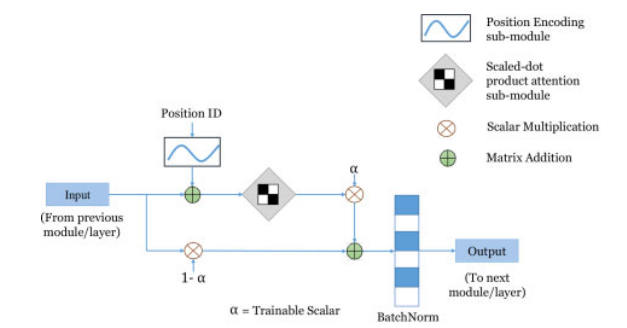
\includegraphics[width=\textwidth]{img1_1.png}
         \caption{}
         \label{fig:the self-attention module }
     \end{subfigure}
     \begin{subfigure}[b]{0.4\textwidth}
         \centering
         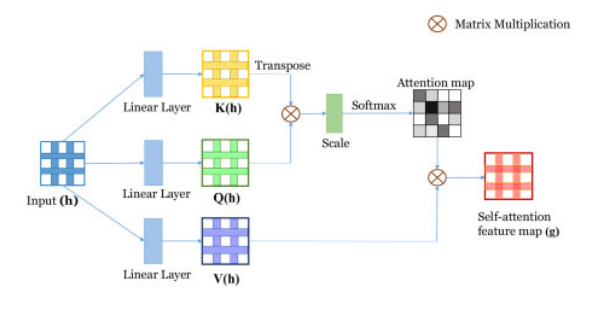
\includegraphics[width=\textwidth]{img1_2.png}
         \caption{}
         \label{fig:caled dot-product attention sub-module.}
     \end{subfigure}
     \begin{subfigure}[b]{0.4\textwidth}
         \centering
         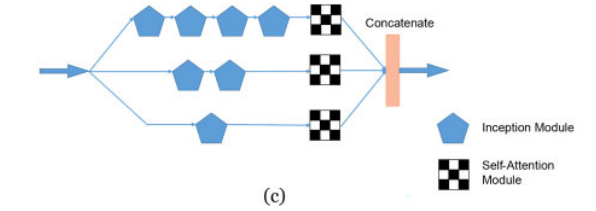
\includegraphics[width=\textwidth]{img1_3.png}
         \caption{}
         \label{fig:Architecture of our proposed 2A3I module}
     \end{subfigure}
     \begin{subfigure}[b]{0.4\textwidth}
         \centering
         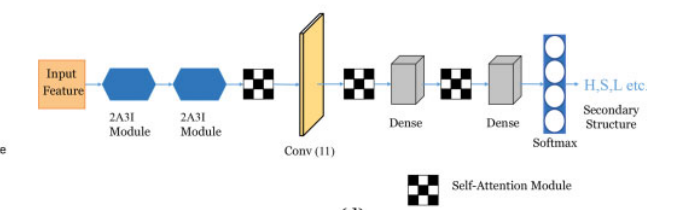
\includegraphics[width=\textwidth]{img1_4.png}
         \caption{}
         \label{fig:overall architecture of SAINT,}
     \end{subfigure}
        \caption{ Schematic diagrams of SAINT and its various components. (a) Architecture of the self-attention module used in SAINT. (b) Architecture of the scaled dot-product attention sub-module. (c) Architecture of our proposed 2A3I module by augmenting self-attention within the 3I network. (d) A schematic diagram of the overall architecture of
SAINT, which comprises two 2A3I modules, three self-attention modules, convolutional layers with window size 11 and 2 dense layers}
        \label{fig:picture1}

\end{figure}


\begin{multicols}{2}
\section{ Results and discussion}
\subsection{Results on benchmark dataset}
The comparison of SAINT with the state-of-the-art Q8 structure
prediction methods on TEST2016, TEST2018, CASP13, CASP12
and CASP-FM is shown in Table 1. To train SAINT and tune necessary hyper-parameters, we have used the same training and validation sets that were used by SPOT-1D. Notably, SPOT-1D is an
ensemble of nine models where each single model uses predicted
contact map in addition to other features. SAINT, on the other
hand, is an ensemble of only four models, three of which take advantage of predicted contact map with different windows sizes.
Experimental results show that SAINT outperforms all other methods across all the test sets. It is worth mentioning that SAINT’s accuracy on the validation set (78.18\%) was also better than that of
SPOT-1D (77.60\%). SPOT-1D’s base model, which does not require contact maps as features is also an ensemble of nine models,
whereas SAINT-base model is a single model. Despite being a single
model, SAINT-base consistently outperformed SPOT-1D base in
TEST2016 and TEST2018. We could not evaluate SPOT-1D base
on CASP12, CASP13 and CASP-FM as it is not publicly available.
From Table 1, it is also evident that SAINT is substantially better
than the other recent methods, namely, NetSurfP-2.0 and
MUFOLD-SS. Even the base model of SAINT consistently outperformed both NetSurfP-2.0 and MUFOLD-SS. The remarkably large
improvement of SAINT over MUFOLD-SS across all the dataset
suggests the advantage of augmenting our proposed self-attention
mechanism in the Deep3I network used in MUFOLD-SS. Statistical
tests (see Table  \ref{tab:2}) suggests that these improvements of SAINT over
other methods are statistically significant   ($ P << 0:05 $).
In addition to the model accuracy, we also investigated the precision, recall and F1-score to obtain better insights on the performances of various methods. Precision, also known as predictivity,
denotes the confidence that can be imposed on a prediction. Recall
signifies how accurately an algorithm can predict a sample from a
particular class. Sometimes an algorithm tends to over-classify
which results into high recall but low precision. On the other hand,
some algorithms tend to under-classify, preserving the precision at
the cost of recall. In order to get an unbiased evaluation of the performance, F1-score is considered to be an appropriate measure and
has been being used for over 25 years in various domains (\cite{prasetijo2017hoax}; \cite{sang2003introduction}). Tables 3–5
show the precision, recall and F1-score on each of the Q8 obtained
by SAINT and other methods. These results suggest that SAINT
achieves better F1-score than other methods on five states (out of
Q8), showing that SAINT produced more balanced and meaningful
results than other methods. SAINT substantially outperforms other
methods on the non-ordinary states (\cite{wang2016protein}), such as I,
G, S and T. However, MUFOLD-SS and SPOT-1D achieved slightly
better F1-score for the ‘B’ and ‘E’ states, respectively. State ‘I’ (phelix) is extremely rare which comprises 7 or more residues and is
present in 15\% of all known protein structures (\cite{ludwiczak2019pipred}). They are very difficult to predict, but mostly found at functionally important regions, such as ligand- and ion-binding sites
(\cite{ludwiczak2019pipred}). Therefore, specialized predictors, such as
PiPred (\cite{ludwiczak2019pipred}), are also available that only predicts

\begin{table}[H]   
\caption{Statistical significance of the Q8 accuracy between SAINT
and other state-of-the-art methods}
\resizebox{\columnwidth}{!}{
\begin{tabular}{llllll}
\hline
Method       & TEST2016 (1213) & TEST2018 (250) & CASP13 (31) & CASP12(49) & CASP-FM(56) \\
\hline 
SPOT-1D      & $8.168e-27$                & $3.893e-5$                              &     0.101       &           0.0345 &   0.0791          \\
NetSurfP-2,0 &                $2.607e-57$                &     $3.258e-18$                          &    0.179         &   $1.55e-6$         &          0.0001 \\
MUFOLD-SS    &                $1.531e-88$                &         $3.145e-21$                      &    0.179         &           $6.51e-5$ & 0.005
         
\end{tabular}
}\hline
  \captionsetup{justification=left}
   

\caption*{Note: : The numbers of protein chains or domains in these datasets are
shown in parentheses. We show the P-values using a Wilcoxon signed-rank
test..}
    \label{tab:2}
\end{table}



the $\pi$ -helix structures. SAINT significantly outperforms SPOT-1D,
NetSurfP-2.0 and MUFOLD-SS in predicting p-helix in TEST2016
dataset by correctly predicting 21 out of 47 ‘I’ states and thus
achieving a recall of 0.45 for this structure. SAINT’s precision for phelix, on the other hand, is 1. This is remarkable considering the
fact that the p-helix specific predictor, PiPred, reports precision and
recall of 0.48 and 0.46, respectively, on a different dataset which
they analyzed in \cite{ludwiczak2019pipred}. However, this comparison
should be taken with a grain of salt since the reported values are on
different test sets.
We analyzed the CASP-FM dataset comprising the FM targets in
the CASP dataset to demonstrate the performance of models on proteins with previously unseen folds. SAINT achieved the best accuracy on CASP-FM, suggesting SAINT’s superiority in predicting
structures of proteins having unseen folds.
While the advantage of utilizing our proposed self-attention
mechanism in the Deep3I framework of MUFOLD-SS is evident
from the significant improvement of SAINT over MUFOLD-SS
across all the dataset analyzed in this study, we further investigated
the efficacy of our proposed attention mechanism in capturing the
long-range interactions. We computed the number of non-local
interactions per residue for each of the 1213 proteins in TEST2016,
and sorted them in an ascending order. Two residues at sequence
position  $i$  and  $j$  are considered to have non-local interaction if they
are at least 20 residues apart  $| i - j | \geq 20$, but <8 A˚ away in terms
of their atomic distances between Ca atoms (\cite{heffernan2017capturing}).
Next, we put them in six equal sized bins b1; b2; ... ; b6 (each containing 202 proteins except for b6, which contains 203 proteins),
where b1 contains the proteins with the lowest level of non-local
interactions and b6 represents the model condition with the highest
level of non-local interactions. We show the Q8 accuracy of SAINTbase and MUFOLD-SS on these model conditions in Table 6 and
Figure \ref{fig:img2}. Note that, instead of our ensemble model, which is more
accurate than our base model, we deliberately show the results for
our single base model, which uses the same feature set as MUFOLDSS, and the only difference between them is the self-attention modules introduced in our architecture.
These results show that the difference in predictive performance
between SAINT-base and MUFOLD-SS significantly increases with
increasing levels of non-local interactions. There is no statistically
significant difference between them on b1, but as we increase the
level of non-local interactions, SAINT becomes significantly more
accurate than MUFOLD-SS and attains the highest level of improvement on b6. This clearly indicates that capturing non-local interactions by self-attention is the key factor in the improvement. We also
performed the same analyses on other methods (see Fig.  \ref{fig:img3}). The
results in Figure \ref{fig:img3}) show that the differences among of these methods
are not that substantial on the model conditions with low levels of
long-range interactions, but the differences become notable as we increase the non-local interactions. SAINT not only achieved the best
accuracy, its improvement over other methods increases with
increasing amount of long-range interactions as well—suggesting
the superiority of our proposed self-attention mechanism compared
to CNNþLSTM (used in NetSurfP-2.0) and CNN







\begin{figure}[H]
         \centering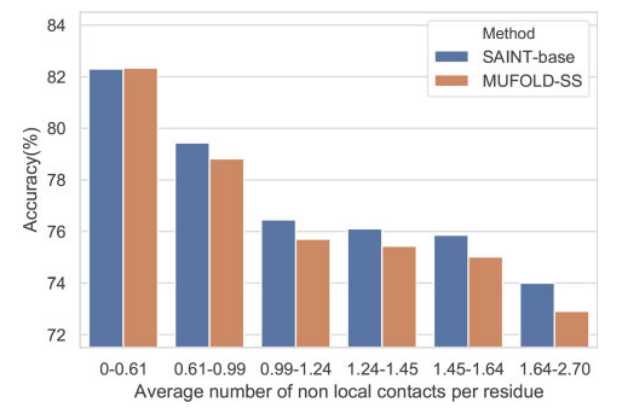
\includegraphics[width=0.5\textwidth]{img2.png}
        
         \caption{Accuracy of SAINT-base and MUFOLD-SS under various levels of non-local
interactions. We show the results on the TEST2016 test set using six bins of proteins as shown in Table 6}
\label{fig:img2}
\end{figure}
\begin{figure}[H]
         \centering
         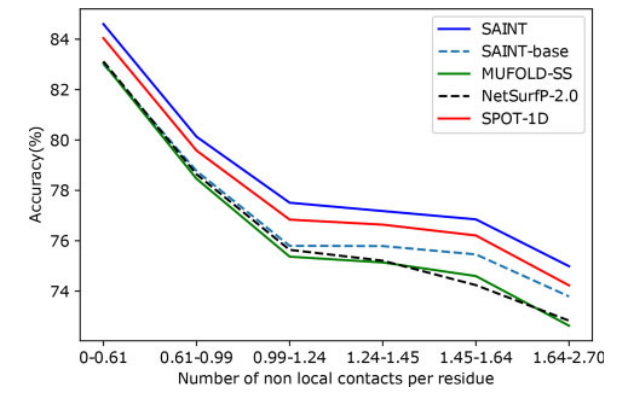
\includegraphics[width=0.5\textwidth]{img3.png}
         \caption{. Accuracy of SAINT, SPOT-1D, NetSurfP-2.0 and MUFOLD-SS as a function
of the average number of non-local interactions per residue. We show the results on
the six bins as shown in Table 6}
\label{fig:img3}
\end{figure}


(ResNet)+BRLSTM (used in SPOT-1D) in terms of capturing the
non-local interactions. In order to demonstrate the efficacy of
SAINT and other methods in capturing the continuous structure of a
protein, we show the 1D map of the annotated and predicted SS of a
representative protein 5M2PA in TEST2016 (see Fig. 4).

\subsection{Running time}
SAINT is much faster than the best alternate method SPOT-1D. For
generating the structures of 1213 protein chains in TEST2016, given
the necessary input files, SAINT took ~360 $\pm $ 5 s whereas SPOT-1D
took ~2485 $\pm $ 5 s on our local machine [Intel core i7-7700 CPU (4
cores), 16 GB RAM, NVIDIA GeForce GTX 1070 GPU]. Under thes ame settings, SAINT took ~197 $\pm $ 5  to generate SSs for the 250
proteins in TEST2018, whereas SPOT-1D took~668 $\pm $ 5  s. Since
both these methods use the same input files for feature generation,
this substantial difference in running time can be attributed to the efficiency of our attention based method over the LSTM networkbased model used in SPOT-1D.

\section{BiblioGraphy}

\bibliography{biblio}
\end{multicols}
\end{document}
